\documentclass[12pt]{article}\usepackage[]{graphicx}\usepackage[svgnames]{xcolor}
%% maxwidth is the original width if it is less than linewidth
%% otherwise use linewidth (to make sure the graphics do not exceed the margin)
\makeatletter
\def\maxwidth{ %
  \ifdim\Gin@nat@width>\linewidth
    \linewidth
  \else
    \Gin@nat@width
  \fi
}
\makeatother

\definecolor{fgcolor}{rgb}{0.345, 0.345, 0.345}
\newcommand{\hlnum}[1]{\textcolor[rgb]{0.686,0.059,0.569}{#1}}%
\newcommand{\hlstr}[1]{\textcolor[rgb]{0.192,0.494,0.8}{#1}}%
\newcommand{\hlcom}[1]{\textcolor[rgb]{0.678,0.584,0.686}{\textit{#1}}}%
\newcommand{\hlopt}[1]{\textcolor[rgb]{0,0,0}{#1}}%
\newcommand{\hlstd}[1]{\textcolor[rgb]{0.345,0.345,0.345}{#1}}%
\newcommand{\hlkwa}[1]{\textcolor[rgb]{0.161,0.373,0.58}{\textbf{#1}}}%
\newcommand{\hlkwb}[1]{\textcolor[rgb]{0.69,0.353,0.396}{#1}}%
\newcommand{\hlkwc}[1]{\textcolor[rgb]{0.333,0.667,0.333}{#1}}%
\newcommand{\hlkwd}[1]{\textcolor[rgb]{0.737,0.353,0.396}{\textbf{#1}}}%
\let\hlipl\hlkwb

\usepackage{framed}
\makeatletter
\newenvironment{kframe}{%
 \def\at@end@of@kframe{}%
 \ifinner\ifhmode%
  \def\at@end@of@kframe{\end{minipage}}%
  \begin{minipage}{\columnwidth}%
 \fi\fi%
 \def\FrameCommand##1{\hskip\@totalleftmargin \hskip-\fboxsep
 \colorbox{shadecolor}{##1}\hskip-\fboxsep
     % There is no \\@totalrightmargin, so:
     \hskip-\linewidth \hskip-\@totalleftmargin \hskip\columnwidth}%
 \MakeFramed {\advance\hsize-\width
   \@totalleftmargin\z@ \linewidth\hsize
   \@setminipage}}%
 {\par\unskip\endMakeFramed%
 \at@end@of@kframe}
\makeatother

\definecolor{shadecolor}{rgb}{.97, .97, .97}
\definecolor{messagecolor}{rgb}{0, 0, 0}
\definecolor{warningcolor}{rgb}{1, 0, 1}
\definecolor{errorcolor}{rgb}{1, 0, 0}
\newenvironment{knitrout}{}{} % an empty environment to be redefined in TeX

\usepackage{alltt}



\usepackage[top=3cm, left=2cm, right=2cm]{geometry} % размер текста на странице

\usepackage[box, % запрет на перенос вопросов
%nopage,
insidebox, % ставим буквы в квадратики
separateanswersheet, % добавляем бланк ответов
nowatermark, % отсутствие надписи "Черновик"
%indivanswers,  % показываем верные ответы
%answers,
lang=RU,
nopage, % убираем оформление страницы (идентификаторы для распознавания)
completemulti]{automultiplechoice}

\usepackage{tikz} % картинки в tikz
\usepackage{microtype} % свешивание пунктуации

\usepackage{dcolumn} % для разделения по десятичной точке (для функции mtable)
\usepackage{comment} % для многострочных комментарией

\usepackage{array} % для столбцов фиксированной ширины

\usepackage{indentfirst} % отступ в первом параграфе

\usepackage{sectsty} % для центрирования названий частей
\allsectionsfont{\centering}

\usepackage{amsmath, amsfonts} % куча стандартных математических плюшек


\usepackage{multicol} % текст в несколько колонок

\usepackage{lastpage} % чтобы узнать номер последней страницы

\usepackage{enumitem} % дополнительные плюшки для списков
%  например \begin{enumerate}[resume] позволяет продолжить нумерацию в новом списке










\usepackage{fancyhdr} % весёлые колонтитулы
\pagestyle{fancy}
\lhead{Эконометрика, промежуточный экзамен}
\chead{}
\rhead{24.12.2016, вариант демо}
\lfoot{}
\cfoot{}
\rfoot{\thepage/\pageref{LastPage}}
\renewcommand{\headrulewidth}{0.4pt}
\renewcommand{\footrulewidth}{0.4pt}



\usepackage{todonotes} % для вставки в документ заметок о том, что осталось сделать
% \todo{Здесь надо коэффициенты исправить}
% \missingfigure{Здесь будет Последний день Помпеи}
% \listoftodos — печатает все поставленные \todo'шки


% более красивые таблицы
\usepackage{booktabs}
% заповеди из докупентации:
% 1. Не используйте вертикальные линни
% 2. Не используйте двойные линии
% 3. Единицы измерения - в шапку таблицы
% 4. Не сокращайте .1 вместо 0.1
% 5. Повторяющееся значение повторяйте, а не говорите "то же"



\usepackage{fontspec}
\usepackage{polyglossia}

\setmainlanguage{russian}
\setotherlanguages{english}

% download "Linux Libertine" fonts:
% http://www.linuxlibertine.org/index.php?id=91&L=1
\setmainfont{Linux Libertine O} % or Helvetica, Arial, Cambria
% why do we need \newfontfamily:
% http://tex.stackexchange.com/questions/91507/
\newfontfamily{\cyrillicfonttt}{Linux Libertine O}

\AddEnumerateCounter{\asbuk}{\russian@alph}{щ} % для списков с русскими буквами


%% эконометрические сокращения
\DeclareMathOperator{\plim}{plim}
\DeclareMathOperator{\Cov}{Cov}
\DeclareMathOperator{\Corr}{Corr}
\DeclareMathOperator{\Var}{Var}
\DeclareMathOperator{\E}{E}
\def \hb{\hat{\beta}}
\def \hs{\hat{\sigma}}
\def \htheta{\hat{\theta}}
\def \s{\sigma}
\def \hy{\hat{y}}
\def \hY{\hat{Y}}
\def \v1{\vec{1}}
\def \e{\varepsilon}
\def \he{\hat{\e}}
\def \z{z}


\def \sVar{\widehat{\Var}}
\def \sCorr{\widehat{\Corr}}
\def \sCov{\widehat{\Cov}}


\def \hVar{\widehat{\Var}}
\def \hCorr{\widehat{\Corr}}
\def \hCov{\widehat{\Cov}}
\def \cN{\mathcal{N}}


\AddEnumerateCounter{\asbuk}{\russian@alph}{щ} % для списков с русскими буквами
\setlist[enumerate, 2]{label=\asbuk*),ref=\asbuk*}
\IfFileExists{upquote.sty}{\usepackage{upquote}}{}
\begin{document}






\element{midterm_demo_16}{ % в фигурных скобках название группы вопросов
%  %\AMCnoCompleteMulti
\begin{questionmult}{1} % тип вопроса (questionmult — множественный выбор) и в фигурных — номер вопроса
В множественной регрессии с константой матрица $X$ имеет размер $56 \times 6$, $TSS=1100$, $ESS=100$. Несмещённая оценка для дисперсии случайных ошибок модели равна
\begin{multicols}{3} % располагаем ответы в 3 колонки
\begin{choices} % опция [o] не рандомизирует порядок ответов
       \correctchoice{$20$}
       \wrongchoice{$18.5$}
       \wrongchoice{$30$}
       \wrongchoice{$\sqrt{30}$}
       \wrongchoice{$\sqrt{40}$}
       \wrongchoice{$40$}
    \end{choices}
   \end{multicols}
\end{questionmult}
}


\element{midterm_demo_16}{ % в фигурных скобках название группы вопросов
 %\AMCnoCompleteMulti
  \begin{questionmult}{2} % тип вопроса (questionmult — множественный выбор) и в фигурных — номер вопроса
  Коэффициент $R^2$ может быть представлен в виде
 \begin{multicols}{2} % располагаем ответы в 3 колонки
   \begin{choices} % опция [o] не рандомизирует порядок ответов
      \correctchoice{$\sum_{j=2}^k \hb_j \frac{\sCov(X_j, Y)}{\sVar(Y)}$}
      \wrongchoice{$\sum_{j=2}^k \hb_j \frac{\sVar(Y)}{\sCov(X_j, Y)}$}
      \wrongchoice{$\sum_{j=2}^k \hb_j \frac{\sCorr(X_j, Y)}{\sVar(Y)}$}
      \wrongchoice{$\sum_{j=2}^k \hb_j \frac{\sCorr(X_j, Y)}{\sVar(\hat Y)}$}
      \wrongchoice{$\sum_{j=2}^k \beta_j \frac{\sCorr(X_j, Y)}{\sVar(\hat Y)}$}
      \wrongchoice{$\sum_{j=2}^k \beta_j \frac{\sVar(Y)}{\sCov(X_j, Y)}$}
   \end{choices}
  \end{multicols}
  \end{questionmult}
}


\element{midterm_demo_16}{ % в фигурных скобках название группы вопросов
 %\AMCnoCompleteMulti
  \begin{questionmult}{3} % тип вопроса (questionmult — множественный выбор) и в фигурных — номер вопроса
    По данным 570 индивидуумов оценили зависимость почасовой оплаты в долларах, $EARN$, от длительности обучения индивидуума в годах, $S$, от результата тестирования индивида в баллах, $ASVABC$, и пола индивидуума, $MALE$, (1 — для мужчин, 0 — для женщин):
\[
\widehat{\ln EARN}_i = \underset{(0.124)}{0.904} +
    \underset{(0.056)}{0.01}S_i + \underset{(0.002)}{0.0157} ASVABC_i + \underset{(0.1)}{0.27} MALE_i
\]
 \begin{multicols}{2} % располагаем ответы в 3 колонки
   \begin{choices} % опция [o] не рандомизирует порядок ответов
      \correctchoice{больше на 27 процентов}
      \wrongchoice{не отличается от оплаты труда женщин}
      \wrongchoice{больше на 0.27 доллара}
      \wrongchoice{больше на 27 долларов}
      \wrongchoice{больше на 0.27 процента}
   \end{choices}
  \end{multicols}
  \end{questionmult}
}


\element{midterm_demo_16}{ % в фигурных скобках название группы вопросов
 %\AMCnoCompleteMulti
  \begin{questionmult}{4} % тип вопроса (questionmult — множественный выбор) и в фигурных — номер вопроса
    Зависимость спроса на некоторый вид услуг $Y$ от его цены $Р$ имеет вид $\hat Y_i = \underset{(2)}{30} - \underset{(0.001)}{0.03} P_i$. Чтобы спрос в среднем снизился на 3\% цена должна увеличиться на
 \begin{multicols}{3} % располагаем ответы в 3 колонки
   \begin{choices} % опция [o] не рандомизирует порядок ответов
      \correctchoice{1 единицу}
      \wrongchoice{100 единиц}
      \wrongchoice{10 единиц }
      \wrongchoice{1\%}
      \wrongchoice{10\%}
   \end{choices}
  \end{multicols}
  \end{questionmult}
}

\element{midterm_demo_16}{ % в фигурных скобках название группы вопросов
 %\AMCnoCompleteMulti
  \begin{questionmult}{5} % тип вопроса (questionmult — множественный выбор) и в фигурных — номер вопроса
    По данным  500 индивидуумов оценили зависимость веса индивидуума $Y$, измеряемого в фунтах (1 фунт $\approx$ 0.5 кг) от его роста $Х$, измеряемого в в футах (1 фут $\approx$ 30 см): $\widehat{\ln Y}_i = -4.4 + 2.4 \ln X_i$. Если рост индивидуума будет измерен в метрах, а вес — в килограммах, то коэффициент перед $\ln X$ будет равен
 \begin{multicols}{3} % располагаем ответы в 3 колонки
   \begin{choices} % опция [o] не рандомизирует порядок ответов
      \correctchoice{$2.4$}
      \wrongchoice{$8$}
      \wrongchoice{$1.2$}
      \wrongchoice{$4.8$}
   \end{choices}
  \end{multicols}
  \end{questionmult}
}

\element{midterm_demo_16}{ % в фигурных скобках название группы вопросов
 %\AMCnoCompleteMulti
  \begin{questionmult}{6} % тип вопроса (questionmult — множественный выбор) и в фигурных — номер вопроса
    Если оценивается модель  $\hat Y_i = \hb_1 + \hb_2 X_i$, а истинной является модель $Y_i = \beta_1 + \beta_2 X_i + \beta_3 Z_i + u_i$, то МНК-оценка $\hb_2$ оказывается
 \begin{multicols}{3} % располагаем ответы в 3 колонки
   \begin{choices} % опция [o] не рандомизирует порядок ответов
      \correctchoice{несмещённой при $\sCov(X, Z) = 0$}
      \wrongchoice{всегда смещённой}
      \wrongchoice{эффективной}
      \wrongchoice{равной нулю}
      \wrongchoice{всегда несмещённой}
      \wrongchoice{несмещённой при $\beta_1 = 0$}
   \end{choices}
  \end{multicols}
  \end{questionmult}
}

\element{midterm_demo_16}{ % в фигурных скобках название группы вопросов
 %\AMCnoCompleteMulti
  \begin{questionmult}{7} % тип вопроса (questionmult — множественный выбор) и в фигурных — номер вопроса
    Если в регрессии отсутствует свободный член, то в общем случае
 \begin{multicols}{2} % располагаем ответы в 3 колонки
   \begin{choices} % опция [o] не рандомизирует порядок ответов
      \correctchoice{$TSS \neq ESS + RSS$}
      \wrongchoice{$R^2$ является мерой качества подгонки регрессии}
      \wrongchoice{сумма остатков равна нулю}
      \wrongchoice{сумма квадратов остатков равна нулю}
      \wrongchoice{$\sum_i \hat Y_i = \sum_i Y_i$}
   \end{choices}
  \end{multicols}
  \end{questionmult}
}

\element{midterm_demo_16}{ % в фигурных скобках название группы вопросов
 %\AMCnoCompleteMulti
  \begin{questionmult}{8} % тип вопроса (questionmult — множественный выбор) и в фигурных — номер вопроса
    На третьем шаге теста МакАлера исследователь получил следующие результаты:
    \[
       \widehat{\ln Y_i} = \underset{(0.20)}{1.54} - \underset{(0.05)}{1.2}X_i + \underset{(0.3)}{3.1}\hat v_{\exp(\widehat{\ln Y}),i}
    \]
    \[
       \hat Y_i = \underset{(0.02)}{1.24} + \underset{(0.03)}{1.1}X_i + \underset{(0.2)}{2.4}\hat v_{\ln \hat Y, i}
    \]


На основании этих результатов исследователь
 %\begin{multicols}{3} % располагаем ответы в 3 колонки
   \begin{choices} % опция [o] не рандомизирует порядок ответов
      \correctchoice{не может выбрать ни логарифмическую, ни линейную модель}
      \wrongchoice{должен предпочесть полулогарифмическую модель}
      \wrongchoice{должен предпочесть линейную модель}
      \wrongchoice{должен отвергнуть гипотезу об адекватности исходной модели}
      \wrongchoice{должен сделать вывод о наличии пропущенных переменных}
      \wrongchoice{должен сделать вывод об отсутствии пропущенных переменных}
   \end{choices}
  %\end{multicols}
  \end{questionmult}
}

\element{midterm_demo_16}{ % в фигурных скобках название группы вопросов
 %\AMCnoCompleteMulti
  \begin{questionmult}{9} % тип вопроса (questionmult — множественный выбор) и в фигурных — номер вопроса
    Известны 95\%-ые доверительные интервалы для коэффициентов регрессии: $\beta_1 \in [-4; 10]$, $\beta_2 \in [2; 10]$. На уровне значимости 5\%
 \begin{multicols}{3} % располагаем ответы в 3 колонки
   \begin{choices} % опция [o] не рандомизирует порядок ответов
      \correctchoice{$\hb_1$ не значим, $\hb_2$ значим}
      \wrongchoice{$\hb_1$ значим, $\hb_2$ значим}
      \wrongchoice{$\hb_1$ значим, $\hb_2$ не значим}
      \wrongchoice{$\hb_1$ не значим, $\hb_2$ не значим}
      \wrongchoice{значимость проверить невозможно}
   \end{choices}
  \end{multicols}
  \end{questionmult}
}

\element{midterm_demo_16}{ % в фигурных скобках название группы вопросов
 %\AMCnoCompleteMulti
  \begin{questionmult}{10} % тип вопроса (questionmult — множественный выбор) и в фигурных — номер вопроса
    Запись $3.20E-16$ означает
 \begin{multicols}{3} % располагаем ответы в 3 колонки
   \begin{choices} % опция [o] не рандомизирует порядок ответов
      \correctchoice{$3.2\cdot 10^{-16}$}
      \wrongchoice{$3.2\cdot e^{-16}$}
      \wrongchoice{$3.2\cdot e - 16$}
      \wrongchoice{$3.2\cdot (e - 16)$}
      \wrongchoice{$3.2^{e-16}$}
      \wrongchoice{Ошибка с кодом 16}
   \end{choices}
  \end{multicols}
  \end{questionmult}
}


%%%%%%%%%%%%%%%%%%%%
















\element{combat_kr_01_16}{ % в фигурных скобках название группы вопросов
 %\AMCnoCompleteMulti
  \begin{questionmult}{pr_01} % тип вопроса (questionmult — множественный выбор) и в фигурных — номер вопроса
    Если $\E(X) = 4$, $\E(Y) = 3$, $\Var(X) = 6$, $\Var(Y) = 7$, $\Cov(X,Y) = -1$, то $\Cov(1 - X + 2Y, 1X)$  равна
 \begin{multicols}{3} % располагаем ответы в 3 колонки
   \begin{choices} % опция [o] не рандомизирует порядок ответов
      \correctchoice{-8}
      \wrongchoice{8}
      \wrongchoice{4}
      \wrongchoice{-4}
      \wrongchoice{-7}
      \wrongchoice{-9}
   \end{choices}
  \end{multicols}
  \end{questionmult}
}

\element{combat_kr_01_16_rejected}{ % в фигурных скобках название группы вопросов
 %\AMCnoCompleteMulti
  \begin{questionmult}{pr_02} % тип вопроса (questionmult — множественный выбор) и в фигурных — номер вопроса
    Джеймс Бонд оценил парную регрессию и оказалось, что $\hat Y_i = 5 + 6 X_i$. Если Джеймс Бонд оценит регрессию без константы, то окажется, что
 \begin{multicols}{3} % располагаем ответы в 3 колонки
   \begin{choices} % опция [o] не рандомизирует порядок ответов
      %\correctchoice{}
      \wrongchoice{$\hat Y_i = 6 X_i$}
      \wrongchoice{$\hat Y_i = 11 X_i$}
      \wrongchoice{$\hat Y_i = 5$}
      \wrongchoice{$\hat Y_i = 11$}
      \wrongchoice{$\hat Y_i = 5.5 X_i$}
      \wrongchoice{$\hat Y_i = 5.5$}
   \end{choices}
  \end{multicols}
  \end{questionmult}
}



\element{combat_kr_01_16}{ % в фигурных скобках название группы вопросов
 %\AMCnoCompleteMulti
  \begin{questionmult}{pr_03} % тип вопроса (questionmult — множественный выбор) и в фигурных — номер вопроса
    Предпосылки теоремы Гаусса-Маркова выполнены, случайные ошибки нормально распределены, уровень доверия равен $80$\%, критическое значение $t$-статистики равно $1.53$, всего $n$ наблюдений. Регрессия имеет вид $\hat Y_i = \underset{(3)}{-4} + \underset{(0.2)}{5}X_i$, в скобках указаны стандартные ошибки. Доверительный интервал для $\beta_2$ равен
 \begin{multicols}{3} % располагаем ответы в 3 колонки
   \begin{choices} % опция [o] не рандомизирует порядок ответов
      \correctchoice{$[4.69; 5.31]$}
      \wrongchoice{$[3.47; 6.53]$}
      \wrongchoice{$[1.94; 8.06]$}
      \wrongchoice{$[4.88; 5.12]$}
      \wrongchoice{$[4.25; 5.75]$}
%      \wrongchoice{не существует}
   \end{choices}
  \end{multicols}
  \end{questionmult}
}

\element{combat_kr_01_16}{ % в фигурных скобках название группы вопросов
 %\AMCnoCompleteMulti
  \begin{questionmult}{pr_04} % тип вопроса (questionmult — множественный выбор) и в фигурных — номер вопроса
    Имеются данные по доходу жены, мужа и продолжительности брака. Доход семьи складывается из дохода жены и мужа. Вася оценил зависимость дохода семьи от продолжительности брака и получил регрессию $\hat Y_i  = 20 + 3X_i$, Петя оценил зависимость дохода мужа от продолжительности брака и получил регрессию $\hat Y_i  = 10 + 2X_i$. Маша оценивает зависимость дохода жены от продолжительности брака. Она получит регрессию:
 \begin{multicols}{2} % располагаем ответы в 3 колонки
   \begin{choices} % опция [o] не рандомизирует порядок ответов
      \correctchoice{$\hat Y_i  = 10+X_i$}
      \wrongchoice{$\hat Y_i  = 10-X_i$}
      \wrongchoice{$\hat Y_i  = 30+5X_i$}
      \wrongchoice{$\hat Y_i  = 20+3X_i$}
      \wrongchoice{$\hat Y_i  = 15+2.5X_i$}
      \wrongchoice{недостаточно данных для ответа}
   \end{choices}
  \end{multicols}
  \end{questionmult}
}

\element{combat_kr_01_16}{ % в фигурных скобках название группы вопросов
 %\AMCnoCompleteMulti
  \begin{questionmult}{pr_05} % тип вопроса (questionmult — множественный выбор) и в фигурных — номер вопроса
    В парной регрессии на уровне значимости 5\%-ов гипотеза $H_0$: $\beta_2 = 2016$ не отвергается. Из этого можно сделать вывод, что на соответствующем уровне значимости
 \begin{multicols}{2} % располагаем ответы в 3 колонки
   \begin{choices} % опция [o] не рандомизирует порядок ответов
      \wrongchoice{$H_0$: $\beta_2 = 0$ отвергается}
      \wrongchoice{$H_0$: $\beta_2 = 0$ не отвергается}
      \wrongchoice{$H_a$: $\beta_2 \neq 0$ не отвергается}
      \wrongchoice{$H_a$: $\beta_2 \neq 0$ отвергается}
      \wrongchoice{доверительный интервал для $\beta_2$ не содержит ноль}
   \end{choices}
  \end{multicols}
  \end{questionmult}
}


\element{combat_kr_01_16}{ % в фигурных скобках название группы вопросов
 %\AMCnoCompleteMulti
  \begin{questionmult}{pr_06} % тип вопроса (questionmult — множественный выбор) и в фигурных — номер вопроса
    В парной регрессии величина $\bar Y - \hat\beta_1 - \hat\beta_2 \bar X$
 \begin{multicols}{2} % располагаем ответы в 3 колонки
   \begin{choices} % опция [o] не рандомизирует порядок ответов
      \correctchoice{равна 0}
      \wrongchoice{равна 1}
      \wrongchoice{равна (-1)}
      \wrongchoice{не существует}
      \wrongchoice{может принимать любое неотрицательное значение}
      \wrongchoice{может принимать любое положительное значение}
   \end{choices}
  \end{multicols}
  \end{questionmult}
}



\element{combat_kr_01_16}{ % в фигурных скобках название группы вопросов
 %\AMCnoCompleteMulti
  \begin{questionmult}{pr_07} % тип вопроса (questionmult — множественный выбор) и в фигурных — номер вопроса
    Условием теоремы Гаусса-Маркова, необходимым для несмещённости оценок коэффициентов регрессии в модели $Y_i = \beta_1 + \beta_2 X_i + u_i$ является
 \begin{multicols}{2} % располагаем ответы в 3 колонки
   \begin{choices} % опция [o] не рандомизирует порядок ответов
      \correctchoice{$\E(u_i)=0$}
      \wrongchoice{гомоскедастичность случайных ошибок}
      \wrongchoice{гетероскедастичность случайных ошибок}
      \wrongchoice{нормальность случайных ошибок}
      \wrongchoice{некоррелированность случайных ошибок}
      \wrongchoice{$\E(u_i)\neq 0$}
   \end{choices}
  \end{multicols}
  \end{questionmult}
}




\element{combat_kr_01_16}{ % в фигурных скобках название группы вопросов
 %\AMCnoCompleteMulti
  \begin{questionmult}{pr_08} % тип вопроса (questionmult — множественный выбор) и в фигурных — номер вопроса
    В модели парной регрессии $R^2 = 0.8$, $TSS = 200$ и $12$ наблюдений. Несмещённая оценка дисперсии случайной ошибки равна
 \begin{multicols}{3} % располагаем ответы в 3 колонки
   \begin{choices} % опция [o] не рандомизирует порядок ответов
      \correctchoice{$4$}
      \wrongchoice{$4.1$}
      \wrongchoice{$4.2$}
      \wrongchoice{$3.8$}
      \wrongchoice{$3.9$}
      \wrongchoice{$4.3$}
   \end{choices}
  \end{multicols}
  \end{questionmult}
}





\element{combat_kr_01_16}{ % в фигурных скобках название группы вопросов
 %\AMCnoCompleteMulti
  \begin{questionmult}{pr_09} % тип вопроса (questionmult — множественный выбор) и в фигурных — номер вопроса
    Если все $Y_i$ в линейной регрессии увеличить в два раза, то оценка $\hat\beta_2$
 \begin{multicols}{2} % располагаем ответы в 3 колонки
   \begin{choices} % опция [o] не рандомизирует порядок ответов
      \correctchoice{помножится на $2$}
      \wrongchoice{помножится на $4$}
      \wrongchoice{поделится на $2$}
      \wrongchoice{поделится на $4$}
      \wrongchoice{не изменится}
      \wrongchoice{изменится в произвольную сторону, в зависимости от $X_i$}
   \end{choices}
  \end{multicols}
  \end{questionmult}
}






\element{combat_kr_01_16}{ % в фигурных скобках название группы вопросов
 %\AMCnoCompleteMulti
  \begin{questionmult}{pr_10} % тип вопроса (questionmult — множественный выбор) и в фигурных — номер вопроса
   Если $\alpha = 0.1$ и $P$-значение равно $0.09$, то
 \begin{multicols}{2} % располагаем ответы в 3 колонки
   \begin{choices} % опция [o] не рандомизирует порядок ответов
      \correctchoice{$H_0$ отвергается}
      \wrongchoice{$H_0$ принимается}
      \wrongchoice{$H_a$ отвергается}
      \wrongchoice{$H_a$ не отвергается}
      \wrongchoice{$H_a$ принимается}
      \wrongchoice{недостаточно информации для ответа}
   \end{choices}
  \end{multicols}
  \end{questionmult}
}



\element{combat_kr_01_16}{ % в фигурных скобках название группы вопросов
 %\AMCnoCompleteMulti
  \begin{questionmult}{pr_11} % тип вопроса (questionmult — множественный выбор) и в фигурных — номер вопроса
    Свободно распространяемым программным обеспечением является
 \begin{multicols}{3} % располагаем ответы в 3 колонки
   \begin{choices} % опция [o] не рандомизирует порядок ответов
      \correctchoice{R}
      \wrongchoice{Excel}
      \wrongchoice{Stata}
      \wrongchoice{Eviews}
      \wrongchoice{SPSS}
      \wrongchoice{Matlab}
   \end{choices}
  \end{multicols}
  \end{questionmult}
}


%%% демо и всякая фигня с прошлого







\element{demo_kr_01_16}{ % в фигурных скобках название группы вопросов
 %\AMCnoCompleteMulti
  \begin{questionmult}{pr1} % тип вопроса (questionmult — множественный выбор) и в фигурных — номер вопроса
    Если $\E(X) = -3$, $\E(Y) = 2$, $\Var(X) = 6$, $\Var(Y) = 7$, $\Cov(X,Y) = -1$, то $\Var(5X + 2Y-1)$  равна
 \begin{multicols}{3} % располагаем ответы в 3 колонки
   \begin{choices} % опция [o] не рандомизирует порядок ответов
      \correctchoice{158}
      \wrongchoice{178}
      \wrongchoice{198}
      \wrongchoice{148}
      \wrongchoice{168}
      \wrongchoice{169}
   \end{choices}
  \end{multicols}
  \end{questionmult}
}

\element{demo_kr_01_16}{ % в фигурных скобках название группы вопросов
 \AMCnoCompleteMulti
  \begin{questionmult}{1} % тип вопроса (questionmult — множественный выбор) и в фигурных — номер вопроса
  При добавлении нового наблюдения
% \begin{multicols}{3} % располагаем ответы в 3 колонки
   \begin{choices} % опция [o] не рандомизирует порядок ответов
      \correctchoice{$TSS$ не уменьшится; $R^2$ может и вырасти, и упасть}
      \wrongchoice{$TSS$ может измениться произвольно; $R^2$ не уменьшится}
      \wrongchoice{$TSS$ не увеличится; $R^2$ не уменьшится}
      \wrongchoice{$TSS$ может измениться произвольно; $R^2$ не увеличиться}
      \wrongchoice{$TSS$ может измениться произвольно; $R^2$ может измениться произвольно}
   \end{choices}
%  \end{multicols}
  \end{questionmult}
}


\element{demo_kr_01_16}{ % в фигурных скобках название группы вопросов
 \AMCnoCompleteMulti
  \begin{questionmult}{2} % тип вопроса (questionmult — множественный выбор) и в фигурных — номер вопроса
  Если в модели парной регрессии $Y_i=\beta_1 + \beta_2 X_i + u_i$ все $X_i$ равны константе $2016$, то оценка $\hat \beta_2$ равна
 \begin{multicols}{3} % располагаем ответы в 3 колонки
   \begin{choices} % опция [o] не рандомизирует порядок ответов
      \wrongchoice{$2016$}
      \wrongchoice{$1/2016$}
      \wrongchoice{$-2016$}
      \wrongchoice{$-1/2016$}
      \wrongchoice{$0$}
      \correctchoice{не существует}
      \end{choices}
  \end{multicols}
  \end{questionmult}
}

\element{demo_kr_01_16}{ % в фигурных скобках название группы вопросов
 \AMCnoCompleteMulti
  \begin{questionmult}{3} % тип вопроса (questionmult — множественный выбор) и в фигурных — номер вопроса
  Если в модели парной регрессии $Y_i=\beta_1 + \beta_2 X_i + u_i$ все $Y_i$ равны константе $2016$, то оценка $\hat \beta_2$ равна
 \begin{multicols}{3} % располагаем ответы в 3 колонки
   \begin{choices} % опция [o] не рандомизирует порядок ответов
      \wrongchoice{$2016$}
      \wrongchoice{$1/2016$}
      \wrongchoice{$-2016$}
      \wrongchoice{$-1/2016$}
      \correctchoice{$0$}
      \wrongchoice{не существует}
      \end{choices}
  \end{multicols}
  \end{questionmult}
}

\element{demo_kr_01_16}{ % в фигурных скобках название группы вопросов
 %\AMCnoCompleteMulti
  \begin{questionmult}{4} % тип вопроса (questionmult — множественный выбор) и в фигурных — номер вопроса
  Квартальные данные о ВВП России за 10 лет являются
 \begin{multicols}{2} % располагаем ответы в 3 колонки
   \begin{choices} % опция [o] не рандомизирует порядок ответов
      \wrongchoice{панельными данными}
      \wrongchoice{перекрестной выборкой}
      \wrongchoice{случайной выборкой}
      \wrongchoice{сходящимся рядом}
      \correctchoice{временным рядом}
      \end{choices}
  \end{multicols}
  \end{questionmult}
}

\element{demo_kr_01_16}{ % в фигурных скобках название группы вопросов
 \AMCnoCompleteMulti
  \begin{questionmult}{5} % тип вопроса (questionmult — множественный выбор) и в фигурных — номер вопроса
Предпосылки теоремы Гаусса-Маркова выполнены, случайные ошибки нормально распределены. Регрессия по 25 наблюдениям имеет вид $\hat Y_i = \underset{(2)}{-1}  + \underset{(0.1)}{4}X_i$. В скобках указаны стандартные ошибки. На уровне значимости $0.05$
 \begin{multicols}{1} % располагаем ответы в 3 колонки
   \begin{choices} % опция [o] не рандомизирует порядок ответов
      \wrongchoice{оба коэффициента значимы}
      \correctchoice{значим только коэффициент наклона}
      \wrongchoice{оба коэффициента незначимы}
      \wrongchoice{недостаточно информации для определения значимости}
      \wrongchoice{значим только свободный член}
      \end{choices}
  \end{multicols}
  \end{questionmult}
}

\element{demo_kr_01_16}{ % в фигурных скобках название группы вопросов
 %\AMCnoCompleteMulti
  \begin{questionmult}{6} % тип вопроса (questionmult — множественный выбор) и в фигурных — номер вопроса
  Если $P$-значение $t$-статистики при проверке значимости коэффициента регрессии равно $0.04$, то этот коэффициент не значим при уровне значимости
 \begin{multicols}{3} % располагаем ответы в 3 колонки
   \begin{choices} % опция [o] не рандомизирует порядок ответов
      \wrongchoice{$0.05$}
      \wrongchoice{$0.95$}
      \wrongchoice{$0.9$}
      \wrongchoice{$0.1$}
      \correctchoice{$0.01$}
      \end{choices}
  \end{multicols}
  \end{questionmult}
}


\element{demo_kr_01_16}{ % в фигурных скобках название группы вопросов
 %\AMCnoCompleteMulti
  \begin{questionmult}{7} % тип вопроса (questionmult — множественный выбор) и в фигурных — номер вопроса
  Регрессия по 25 наблюдениям имеет вид $\hat Y_i = \underset{(2)}{-1}  - \underset{(0.5)}{1.5}X_i$. В скобках указаны стандартные ошибки. При проверке гипотезы о равенстве коэффициента наклона $(-1)$ расчётное значение $t$-статистики равно
 \begin{multicols}{3} % располагаем ответы в 3 колонки
   \begin{choices} % опция [o] не рандомизирует порядок ответов
      \wrongchoice{$-2$}
      \wrongchoice{$0.5$}
      \wrongchoice{$2$}
      \wrongchoice{$-0.5$}
      \correctchoice{$-1$}
      \end{choices}
  \end{multicols}
  \end{questionmult}
}


\element{demo_kr_01_16}{ % в фигурных скобках название группы вопросов
 \AMCnoCompleteMulti
  \begin{questionmult}{8} % тип вопроса (questionmult — множественный выбор) и в фигурных — номер вопроса
  В регрессии с константой, оценённой с помощью МНК, сумма остатков
 \begin{multicols}{2} % располагаем ответы в 3 колонки
   \begin{choices} % опция [o] не рандомизирует порядок ответов
      \wrongchoice{может принимать любое неположитлеьное значение}
      \wrongchoice{может принимать любое положительное значение}
      \wrongchoice{может принимать любое значение из $\mathbb{R}$}
      \wrongchoice{равна $1$}
      \correctchoice{равна $0$}
      \wrongchoice{не существует}
      \end{choices}
  \end{multicols}
  \end{questionmult}
}


\element{demo_kr_01_16_rejected}{ % в фигурных скобках название группы вопросов
 \AMCnoCompleteMulti
  \begin{questionmult}{9} % тип вопроса (questionmult — множественный выбор) и в фигурных — номер вопроса
  Если в регрессии с константой, оценённой с помощью МНК, сумма квадратов остатков равна нулю, то показатель $R^2$
 \begin{multicols}{2} % располагаем ответы в 3 колонки
   \begin{choices} % опция [o] не рандомизирует порядок ответов
      \wrongchoice{равен $0$}
      \wrongchoice{равен $-1$}
      \wrongchoice{не существует}
      \wrongchoice{может принимать любое значение на $[0;1]$}
      \correctchoice{равен $1$}
      \wrongchoice{не существует}
      \end{choices}
  \end{multicols}
  \end{questionmult}
}

\element{demo_kr_01_16}{ % в фигурных скобках название группы вопросов
 %\AMCnoCompleteMulti
  \begin{questionmult}{10} % тип вопроса (questionmult — множественный выбор) и в фигурных — номер вопроса
  Необходимым условием теоремы Гаусса-Маркова является
 \begin{multicols}{2} % располагаем ответы в 3 колонки
   \begin{choices} % опция [o] не рандомизирует порядок ответов
      \wrongchoice{наличие в матрице $X$ единичного столбца}
      \wrongchoice{нормальность остатков}
      \wrongchoice{нормальность $Y_i$}
      \wrongchoice{постоянство дисперсии остатков}
      \correctchoice{постоянство дисперсии случайной ошибки}
      \end{choices}
  \end{multicols}
  \end{questionmult}
}




\element{demo_15}{ % в фигурных скобках название группы вопросов
 \AMCnoCompleteMulti
  \begin{questionmult}{1} % тип вопроса (questionmult — множественный выбор) и в фигурных — номер вопроса
  При добавлении новой переменной скорректированный $R^2$
% \begin{multicols}{3} % располагаем ответы в 3 колонки
   \begin{choices} % опция [o] не рандомизирует порядок ответов
      \wrongchoice{обязательно вырастет}
      \wrongchoice{обязательно упадёт}
       \correctchoice{может как вырасти, так и упасть}
      \end{choices}
%  \end{multicols}
  \end{questionmult}
}


\element{demo_15}{ % в фигурных скобках название группы вопросов
 \AMCnoCompleteMulti
  \begin{questionmult}{2} % тип вопроса (questionmult — множественный выбор) и в фигурных — номер вопроса
  При добавлении новой переменной коэффициент детерминации $R^2$:
% \begin{multicols}{3} % располагаем ответы в 3 колонки
   \begin{choices} % опция [o] не рандомизирует порядок ответов
      \correctchoice{обязательно вырастет}
      \wrongchoice{обязательно упадёт}
      \wrongchoice{может как вырасти, так и упасть}
      \end{choices}
%  \end{multicols}
  \end{questionmult}
}


\element{demo_15}{ % в фигурных скобках название группы вопросов
 \AMCnoCompleteMulti
  \begin{questionmult}{3} % тип вопроса (questionmult — множественный выбор) и в фигурных — номер вопроса
  Для проверки гипотезы о значимости коэффициентов при мультиколлинеарности стандартные $t$-статистики
% \begin{multicols}{3} % располагаем ответы в 3 колонки
   \begin{choices} % опция [o] не рандомизирует порядок ответов
      \correctchoice{можно использовать, т.к. они по прежнему имеют $t$-распределение}
      \wrongchoice{нельзя использовать т.к. они не имеют $t$-распределения}
      \end{choices}
%  \end{multicols}
  \end{questionmult}
}

\element{demo_15}{ % в фигурных скобках название группы вопросов
 \AMCnoCompleteMulti
  \begin{questionmult}{4} % тип вопроса (questionmult — множественный выбор) и в фигурных — номер вопроса
  При условной гетероскедастичности и наблюдениях, представляющих случайную выборку, оценки МНК
 \begin{multicols}{2} % располагаем ответы в 3 колонки
   \begin{choices} % опция [o] не рандомизирует порядок ответов
      \correctchoice{остаются состоятельными}
      \wrongchoice{перестают быть состоятельными}
      \end{choices}
  \end{multicols}
  \end{questionmult}
}


\element{demo_15}{ % в фигурных скобках название группы вопросов
 \AMCnoCompleteMulti
  \begin{questionmult}{5} % тип вопроса (questionmult — множественный выбор) и в фигурных — номер вопроса
  При условной гетероскедастичности и наблюдениях, представляющих случайную выборку, оценки МНК
 \begin{multicols}{2} % располагаем ответы в 3 колонки
   \begin{choices} % опция [o] не рандомизирует порядок ответов
      \correctchoice{остаются несмещёнными}
      \wrongchoice{перестают быть несмещёнными}
      \end{choices}
  \end{multicols}
  \end{questionmult}
}


\element{demo_15}{ % в фигурных скобках название группы вопросов
 \AMCnoCompleteMulti
  \begin{questionmult}{6} % тип вопроса (questionmult — множественный выбор) и в фигурных — номер вопроса
  При предпосылке о нормально распределенных ошибках в классической линейной регрессионной модели оценки коэффициентов уравнения с помощью МНК и оценки с помощью максимального правдоподобия
% \begin{multicols}{3} % располагаем ответы в 3 колонки
   \begin{choices} % опция [o] не рандомизирует порядок ответов
      \correctchoice{совпадают}
      \wrongchoice{отличаются}
      \end{choices}
%  \end{multicols}
  \end{questionmult}
}

\element{demo_15}{ % в фигурных скобках название группы вопросов
 \AMCcompleteMulti
  \begin{questionmult}{7} % тип вопроса (questionmult — множественный выбор) и в фигурных — номер вопроса
  При условной гетероскедастичности использование робастных стандартных ошибок позволяет
% \begin{multicols}{3} % располагаем ответы в 3 колонки
   \begin{choices} % опция [o] не рандомизирует порядок ответов
      \wrongchoice{устранить смещённость оценок коэффициентов}
      \wrongchoice{устранить несостоятельность оценок коэффициентов}
      \end{choices}
%  \end{multicols}
  \end{questionmult}
}

\element{demo_15}{ % в фигурных скобках название группы вопросов
 \AMCcompleteMulti
  \begin{questionmult}{8} % тип вопроса (questionmult — множественный выбор) и в фигурных — номер вопроса
  При автокорреляции первого порядка в ошибках использование робастных стандартных ошибок Нью-Веста позволяет
% \begin{multicols}{3} % располагаем ответы в 3 колонки
   \begin{choices} % опция [o] не рандомизирует порядок ответов
     \wrongchoice{устранить смещённость оценок коэффициентов}
     \wrongchoice{устранить несостоятельность оценок коэффициентов}
      \end{choices}
%  \end{multicols}
  \end{questionmult}
}

\element{demo_15}{ % в фигурных скобках название группы вопросов
 \AMCnoCompleteMulti
  \begin{questionmult}{9} % тип вопроса (questionmult — множественный выбор) и в фигурных — номер вопроса
  Если нарушена только предпосылка $\E(u_i) = 0$, то при оценке модели $y_i = \beta_1 + \beta_2 x_i + u_i$ оценка $\hat \beta_2$ окажется
 \begin{multicols}{2} % располагаем ответы в 3 колонки
   \begin{choices} % опция [o] не рандомизирует порядок ответов
      \correctchoice{несмещённой}
      \wrongchoice{смещённой}
      \end{choices}
 \end{multicols}
  \end{questionmult}
}


\element{demo_15}{ % в фигурных скобках название группы вопросов
 \AMCnoCompleteMulti
  \begin{questionmult}{10} % тип вопроса (questionmult — множественный выбор) и в фигурных — номер вопроса
  Если все выборочные корреляции между регрессорами по модулю меньше 0.1 то строгая мультиколлинеарность
 \begin{multicols}{2} % располагаем ответы в 3 колонки
   \begin{choices} % опция [o] не рандомизирует порядок ответов
      \correctchoice{возможна}
      \wrongchoice{невозможна}
      \end{choices}
 \end{multicols}
  \end{questionmult}
}




















\element{combat_15}{ % в фигурных скобках название группы вопросов
 \AMCcompleteMulti
  \begin{questionmult}{1} % тип вопроса (questionmult — множественный выбор) и в фигурных — номер вопроса
  Предпосылка об отсутствии систематической ошибки в модели означает, что для всех наблюдений
 \begin{multicols}{2} % располагаем ответы в 3 колонки
   \begin{choices} % опция [o] не рандомизирует порядок ответов
      \wrongchoice{$\Var(\varepsilon_i)=0$}
      \wrongchoice{$\Var(\varepsilon_i) \neq 0$}
      \end{choices}
  \end{multicols}
  \end{questionmult}
}

\element{combat_15}{ % в фигурных скобках название группы вопросов
 \AMCnoCompleteMulti
  \begin{questionmult}{2} % тип вопроса (questionmult — множественный выбор) и в фигурных — номер вопроса
  Стандартные ошибки в форме Уайта в случае гетероскедастичности помогают устранить несостоятельность оценок коэффициентов
 \begin{multicols}{2} % располагаем ответы в 3 колонки
   \begin{choices} % опция [o] не рандомизирует порядок ответов
      \correctchoice{неверно}
      \wrongchoice{верно}
      \end{choices}
  \end{multicols}
  \end{questionmult}
}

\element{combat_15}{ % в фигурных скобках название группы вопросов
 \AMCnoCompleteMulti
  \begin{questionmult}{3} % тип вопроса (questionmult — множественный выбор) и в фигурных — номер вопроса
  Незначимость всех коэффициентов регрессии
 \begin{multicols}{2} % располагаем ответы в 3 колонки
   \begin{choices} % опция [o] не рандомизирует порядок ответов
      \correctchoice{может быть не связана с мультиколлинеарностью}
      \wrongchoice{обязательно свидетельствует о наличии мультиколлинеарности}
      \end{choices}
  \end{multicols}
  \end{questionmult}
}


\element{combat_15}{ % в фигурных скобках название группы вопросов
 \AMCnoCompleteMulti
  \begin{questionmult}{4} % тип вопроса (questionmult — множественный выбор) и в фигурных — номер вопроса
  После применения МНК к модели $y_i=\beta x_i + \varepsilon_i$   сумма $ESS+RSS$
 \begin{multicols}{2} % располагаем ответы в 3 колонки
   \begin{choices} % опция [o] не рандомизирует порядок ответов
      \correctchoice{может быть не равна $TSS$}
      \wrongchoice{обязательно равна $TSS$}
      \end{choices}
  \end{multicols}
  \end{questionmult}
}

\element{combat_15}{ % в фигурных скобках название группы вопросов
 \AMCnoCompleteMulti
  \begin{questionmult}{5} % тип вопроса (questionmult — множественный выбор) и в фигурных — номер вопроса
  При наличии ошибок измерения зависимой переменной МНК-оценки коэффициентов модели
 \begin{multicols}{2} % располагаем ответы в 3 колонки
   \begin{choices} % опция [o] не рандомизирует порядок ответов
      \correctchoice{состоятельны}
      \wrongchoice{несостоятельны}
      \end{choices}
  \end{multicols}
  \end{questionmult}
}

\element{combat_15}{ % в фигурных скобках название группы вопросов
 \AMCnoCompleteMulti
  \begin{questionmult}{6} % тип вопроса (questionmult — множественный выбор) и в фигурных — номер вопроса
  Если выполнены все предпосылки теоремы Гаусса-Маркова, но остатки модели не подчиняются нормальному закону распределения, то МНК-оценки коэффициентов регрессии являются
 \begin{multicols}{2} % располагаем ответы в 3 колонки
   \begin{choices} % опция [o] не рандомизирует порядок ответов
      \correctchoice{несмещёнными}
      \wrongchoice{смещёнными}
      \end{choices}
  \end{multicols}
  \end{questionmult}
}


\element{combat_15}{ % в фигурных скобках название группы вопросов
 \AMCnoCompleteMulti
  \begin{questionmult}{7} % тип вопроса (questionmult — множественный выбор) и в фигурных — номер вопроса
  Индексы вздутия дисперсии (VIF) в случае отсутствия мультиколлинеарности лежат в интервале
 \begin{multicols}{2} % располагаем ответы в 3 колонки
   \begin{choices} % опция [o] не рандомизирует порядок ответов
      \correctchoice{$[1;+\infty)$}
      \wrongchoice{$[0;1]$}
      \end{choices}
  \end{multicols}
  \end{questionmult}
}


\element{combat_15}{ % в фигурных скобках название группы вопросов
 \AMCnoCompleteMulti
  \begin{questionmult}{8} % тип вопроса (questionmult — множественный выбор) и в фигурных — номер вопроса
  Нулевая гипотеза в тесте Дарбина-Уотсона состоит в
 \begin{multicols}{2} % располагаем ответы в 3 колонки
   \begin{choices} % опция [o] не рандомизирует порядок ответов
      \correctchoice{отсутствии автокорреляции}
      \wrongchoice{наличии автокорреляции}
      \end{choices}
  \end{multicols}
  \end{questionmult}
}

\element{combat_15}{ % в фигурных скобках название группы вопросов
 \AMCnoCompleteMulti
  \begin{questionmult}{9} % тип вопроса (questionmult — множественный выбор) и в фигурных — номер вопроса
  Если в модель добавили незначимый фактор, то коэффициент детерминации $R^2$
 \begin{multicols}{3} % располагаем ответы в 3 колонки
   \begin{choices} % опция [o] не рандомизирует порядок ответов
      \correctchoice{вырастет}
      \wrongchoice{упадёт}
      \wrongchoice{не изменится}
      \end{choices}
  \end{multicols}
  \end{questionmult}
}

\element{combat_15}{ % в фигурных скобках название группы вопросов
 \AMCnoCompleteMulti
  \begin{questionmult}{10} % тип вопроса (questionmult — множественный выбор) и в фигурных — номер вопроса
  При диагностике автокорреляции третьего порядка тест Бройша-Годфри
 \begin{multicols}{3} % располагаем ответы в 3 колонки
   \begin{choices} % опция [o] не рандомизирует порядок ответов
      \correctchoice{применим}
      \wrongchoice{неприменим}
      \end{choices}
  \end{multicols}
  \end{questionmult}
}


\element{combat_15_v2}{ % в фигурных скобках название группы вопросов
 \AMCnoCompleteMulti
  \begin{questionmult}{11} % тип вопроса (questionmult — множественный выбор) и в фигурных — номер вопроса
  Нормальность остатков является одной из предпосылок теоремы Гаусса-Маркова
 \begin{multicols}{3} % располагаем ответы в 3 колонки
   \begin{choices} % опция [o] не рандомизирует порядок ответов
      \correctchoice{неверно}
      \wrongchoice{верно}
      \end{choices}
  \end{multicols}
  \end{questionmult}
}


\element{combat_15_v2}{ % в фигурных скобках название группы вопросов
 \AMCcompleteMulti
  \begin{questionmult}{12} % тип вопроса (questionmult — множественный выбор) и в фигурных — номер вопроса
  В случае гетероскедастичности применение стандартных ошибок в форме Уайта позволяет сделать оценки коэффициентов регрессии
 \begin{multicols}{3} % располагаем ответы в 3 колонки
   \begin{choices} % опция [o] не рандомизирует порядок ответов
      \wrongchoice{несмещёнными}
      \wrongchoice{состоятельными}
      \wrongchoice{эффективными}
      \end{choices}
  \end{multicols}
  \end{questionmult}
}

\element{combat_15_v2}{ % в фигурных скобках название группы вопросов
 \AMCnoCompleteMulti
  \begin{questionmult}{13} % тип вопроса (questionmult — множественный выбор) и в фигурных — номер вопроса
  С помощью МНК оценивается модель $y_i = \beta_1 + \beta_2 x_i + \varepsilon_i$. Наблюдения представляют собой случайную выборку, и $\Cov(\varepsilon_i, x_i) = 1$. В этом случае $\plim \hat \beta_2^{ols}$
 \begin{multicols}{3} % располагаем ответы в 3 колонки
   \begin{choices} % опция [o] не рандомизирует порядок ответов
      \correctchoice{не равен $\beta_2$}
      \wrongchoice{равен $\beta_2$}
      \end{choices}
  \end{multicols}
  \end{questionmult}
}


\element{combat_15_v2}{ % в фигурных скобках название группы вопросов
 \AMCnoCompleteMulti
  \begin{questionmult}{14} % тип вопроса (questionmult — множественный выбор) и в фигурных — номер вопроса
  После применения МНК к модели $y_i=\beta x_i+\varepsilon_i$ сумма остатков $\sum \hat \varepsilon_i$
 \begin{multicols}{3} % располагаем ответы в 3 колонки
   \begin{choices} % опция [o] не рандомизирует порядок ответов
      \correctchoice{не равна нулю}
      \wrongchoice{равна нулю}
      \end{choices}
  \end{multicols}
  \end{questionmult}
}

\element{combat_15_v2}{ % в фигурных скобках название группы вопросов
 \AMCnoCompleteMulti
  \begin{questionmult}{15} % тип вопроса (questionmult — множественный выбор) и в фигурных — номер вопроса
  В результате применения МНК к модели $y_i=\beta_1 + \beta_2 x_i+\varepsilon_i$ сумма $\sum x_i \hat \varepsilon_i$
 \begin{multicols}{3} % располагаем ответы в 3 колонки
   \begin{choices} % опция [o] не рандомизирует порядок ответов
      \correctchoice{обязательно равна нулю}
      \wrongchoice{может быть не равна нулю}
      \end{choices}
  \end{multicols}
  \end{questionmult}
}

\element{combat_15_v2}{ % в фигурных скобках название группы вопросов
 \AMCnoCompleteMulti
  \begin{questionmult}{16} % тип вопроса (questionmult — множественный выбор) и в фигурных — номер вопроса
  В случае мультиколлинеарности применение гребневой регрессии (ridge-regression) делает оценки коэффициентов
 \begin{multicols}{3} % располагаем ответы в 3 колонки
   \begin{choices} % опция [o] не рандомизирует порядок ответов
      \correctchoice{смещёнными}
      \wrongchoice{несмещёнными}
      \end{choices}
  \end{multicols}
  \end{questionmult}
}

\element{combat_15_v2}{ % в фигурных скобках название группы вопросов
 \AMCnoCompleteMulti
  \begin{questionmult}{17} % тип вопроса (questionmult — множественный выбор) и в фигурных — номер вопроса
  В случае мультиколлинеарности оценки дисперсий коэффициентов модели становятся
 \begin{multicols}{3} % располагаем ответы в 3 колонки
   \begin{choices} % опция [o] не рандомизирует порядок ответов
      \correctchoice{несмещёнными}
      \wrongchoice{смещёнными}
      \end{choices}
  \end{multicols}
  \end{questionmult}
}

\element{combat_15_v2}{ % в фигурных скобках название группы вопросов
 \AMCcompleteMulti
  \begin{questionmult}{18} % тип вопроса (questionmult — множественный выбор) и в фигурных — номер вопроса
  После применения МНК к исходной модели дополнительно можно оценить модель $\ln(\hat \varepsilon_i^2 )=\gamma_1 + \gamma_2 \ln(x_i) + u_i$  для диагностики
 \begin{multicols}{2} % располагаем ответы в 3 колонки
   \begin{choices} % опция [o] не рандомизирует порядок ответов
      \correctchoice{гетероскедастичности}
      \wrongchoice{автокорреляции}
      \wrongchoice{мультиколлинеарности}
      \end{choices}
  \end{multicols}
  \end{questionmult}
}

\element{combat_15_v2}{ % в фигурных скобках название группы вопросов
 \AMCcompleteMulti
  \begin{questionmult}{19} % тип вопроса (questionmult — множественный выбор) и в фигурных — номер вопроса
  Для сравнения качества моделей $y_i=\beta_1+ \beta_2 x_i+\varepsilon_i$ и $\ln(y_i)=\gamma_1+ \gamma_2 x_i + \varepsilon_i$, оцененных на одном наборе данных, используют
 \begin{multicols}{2} % располагаем ответы в 3 колонки
   \begin{choices} % опция [o] не рандомизирует порядок ответов
      \wrongchoice{коэффициент детерминации $R^2$}
      \wrongchoice{скорректированный коэффициент $R_{adj}^2$}
      \end{choices}
  \end{multicols}
  \end{questionmult}
}


\element{combat_15_v2}{ % в фигурных скобках название группы вопросов
 \AMCnoCompleteMulti
  \begin{questionmult}{20} % тип вопроса (questionmult — множественный выбор) и в фигурных — номер вопроса
  При диагностике автокорреляции первого порядка тест Бройша-Годфри
 \begin{multicols}{2} % располагаем ответы в 3 колонки
   \begin{choices} % опция [o] не рандомизирует порядок ответов
      \correctchoice{применим}
      \wrongchoice{неприменим}
      \end{choices}
  \end{multicols}
  \end{questionmult}
}




















\element{combat_15_v3}{ % в фигурных скобках название группы вопросов
 \AMCnoCompleteMulti
  \begin{questionmult}{1} % тип вопроса (questionmult — множественный выбор) и в фигурных — номер вопроса
  Ошибки измерения независимой переменной являются одной из причин
 \begin{multicols}{2} % располагаем ответы в 3 колонки
   \begin{choices} % опция [o] не рандомизирует порядок ответов
      \correctchoice{эндогенности}
      \wrongchoice{мультиколлинеарности}
      \wrongchoice{автокорреляции}
      \end{choices}
  \end{multicols}
  \end{questionmult}
}

\element{combat_15_v3}{ % в фигурных скобках название группы вопросов
 \AMCnoCompleteMulti
  \begin{questionmult}{2} % тип вопроса (questionmult — множественный выбор) и в фигурных — номер вопроса
  Во временных рядах гетероскедастичность
 \begin{multicols}{2} % располагаем ответы в 3 колонки
   \begin{choices} % опция [o] не рандомизирует порядок ответов
      \correctchoice{возможна}
      \wrongchoice{невозможна}
      \end{choices}
  \end{multicols}
  \end{questionmult}
}

\element{combat_15_v3}{ % в фигурных скобках название группы вопросов
 \AMCnoCompleteMulti
  \begin{questionmult}{3} % тип вопроса (questionmult — множественный выбор) и в фигурных — номер вопроса
  Оценка $\hb$ называется несмещённой, если с ростом числа наблюдений она стремится к истинной $\beta$
 \begin{multicols}{2} % располагаем ответы в 3 колонки
   \begin{choices} % опция [o] не рандомизирует порядок ответов
      \correctchoice{неверно}
      \wrongchoice{верно}
      \end{choices}
  \end{multicols}
  \end{questionmult}
}


\element{combat_15_v3}{ % в фигурных скобках название группы вопросов
 \AMCnoCompleteMulti
  \begin{questionmult}{4} % тип вопроса (questionmult — множественный выбор) и в фигурных — номер вопроса
  С ростом числа наблюдений распределение статистики Дарбина-Уотсона стремится к
 \begin{multicols}{2} % располагаем ответы в 3 колонки
   \begin{choices} % опция [o] не рандомизирует порядок ответов
      \correctchoice{особому распределению Дарбина-Уотсона}
      \wrongchoice{стандартному нормальному распределению}
      \end{choices}
  \end{multicols}
  \end{questionmult}
}

\element{combat_15_v3}{ % в фигурных скобках название группы вопросов
 \AMCcompleteMulti
  \begin{questionmult}{5} % тип вопроса (questionmult — множественный выбор) и в фигурных — номер вопроса
  Одним из способов борьбы с нестрогой мультиколлинеарностью является
 %\begin{multicols}{2} % располагаем ответы в 3 колонки
   \begin{choices} % опция [o] не рандомизирует порядок ответов
      \correctchoice{увеличение количества наблюдений}
      \wrongchoice{деление всех регрессоров на одно и то же большое число}
      \wrongchoice{использование взвешенного МНК}
    \end{choices}
 %\end{multicols}
  \end{questionmult}
}

\element{combat_15_v3}{ % в фигурных скобках название группы вопросов
 \AMCnoCompleteMulti
  \begin{questionmult}{6} % тип вопроса (questionmult — множественный выбор) и в фигурных — номер вопроса
 Нестрогая мультиколлинеарность нарушает теорему Гаусса-Маркова
 \begin{multicols}{2} % располагаем ответы в 3 колонки
   \begin{choices} % опция [o] не рандомизирует порядок ответов
      \correctchoice{неверно}
      \wrongchoice{верно}
      \end{choices}
  \end{multicols}
  \end{questionmult}
}


\element{combat_15_v3}{ % в фигурных скобках название группы вопросов
 \AMCnoCompleteMulti
  \begin{questionmult}{7} % тип вопроса (questionmult — множественный выбор) и в фигурных — номер вопроса
  Если ошибки распределены не нормально, то МНК-оценки коэффициентов регрессии
 \begin{multicols}{2} % располагаем ответы в 3 колонки
   \begin{choices} % опция [o] не рандомизирует порядок ответов
      \correctchoice{эффективны и несмещены}
      \wrongchoice{неэффективны и смещены}
      \wrongchoice{эффективны и смещены}
      \wrongchoice{неэффективны и несмещены}
    \end{choices}
  \end{multicols}
  \end{questionmult}
}


\element{combat_15_v3}{ % в фигурных скобках название группы вопросов
 \AMCnoCompleteMulti
  \begin{questionmult}{8} % тип вопроса (questionmult — множественный выбор) и в фигурных — номер вопроса
 Если в модели присутствуют лаги независимой переменной, то тест Дарбина-Уотсона
 \begin{multicols}{2} % располагаем ответы в 3 колонки
   \begin{choices} % опция [o] не рандомизирует порядок ответов
      \correctchoice{применим}
      \wrongchoice{неприменим}
      \end{choices}
  \end{multicols}
  \end{questionmult}
}

\element{combat_15_v3}{ % в фигурных скобках название группы вопросов
 \AMCnoCompleteMulti
  \begin{questionmult}{9} % тип вопроса (questionmult — множественный выбор) и в фигурных — номер вопроса
  При гетероскедастичности оценки коэффициентов
 \begin{multicols}{2} % располагаем ответы в 3 колонки
   \begin{choices} % опция [o] не рандомизирует порядок ответов
      \correctchoice{остаются несмещёнными}
      \wrongchoice{в среднем завышены}
      \wrongchoice{в среднем занижены}
      \end{choices}
  \end{multicols}
  \end{questionmult}
}

\element{combat_15_v3}{ % в фигурных скобках название группы вопросов
 \AMCnoCompleteMulti
  \begin{questionmult}{10} % тип вопроса (questionmult — множественный выбор) и в фигурных — номер вопроса
  У разностного  уравнения $y_t=0.1y_{t-1} + \e_t +0.4\e_{t-1}$
 \begin{multicols}{3} % располагаем ответы в 3 колонки
   \begin{choices} % опция [o] не рандомизирует порядок ответов
      \correctchoice{есть единственное стационарное решение}
      \wrongchoice{нет стационарных решений}
      \wrongchoice{есть бесконечное количество стационарных решений}
    \end{choices}
  \end{multicols}
  \end{questionmult}
}























\element{combat_15_v4}{ % в фигурных скобках название группы вопросов
 \AMCcompleteMulti
  \begin{questionmult}{1} % тип вопроса (questionmult — множественный выбор) и в фигурных — номер вопроса
  В теореме Гаусса-Маркова предполагается, что ошибки
 \begin{multicols}{2} % располагаем ответы в 3 колонки
   \begin{choices} % опция [o] не рандомизирует порядок ответов
      \wrongchoice{имеют нулевое математическое ожидание и единичную дисперсию}
      \wrongchoice{имеют ненулевое математическое ожидание и неединичную дисперсию}
    \end{choices}
  \end{multicols}
  \end{questionmult}
}

\element{combat_15_v4}{ % в фигурных скобках название группы вопросов
 \AMCnoCompleteMulti
  \begin{questionmult}{2} % тип вопроса (questionmult — множественный выбор) и в фигурных — номер вопроса
  При условной гетероскедастичности оценки коэффициентов
 \begin{multicols}{2} % располагаем ответы в 3 колонки
   \begin{choices} % опция [o] не рандомизирует порядок ответов
      \correctchoice{состоятельны}
      \wrongchoice{несостоятельны}
      \end{choices}
  \end{multicols}
  \end{questionmult}
}

\element{combat_15_v4}{ % в фигурных скобках название группы вопросов
 \AMCcompleteMulti
  \begin{questionmult}{3} % тип вопроса (questionmult — множественный выбор) и в фигурных — номер вопроса
  Двухшаговый метод наименьших квадратов — это стандартный способ борьбы с
 \begin{multicols}{2} % располагаем ответы в 3 колонки
   \begin{choices} % опция [o] не рандомизирует порядок ответов
      \correctchoice{эндогенностью}
      \wrongchoice{автокорреляцией}
      \wrongchoice{гетероскедастичностью}
      \end{choices}
  \end{multicols}
  \end{questionmult}
}


\element{combat_15_v4}{ % в фигурных скобках название группы вопросов
 \AMCnoCompleteMulti
  \begin{questionmult}{4} % тип вопроса (questionmult — множественный выбор) и в фигурных — номер вопроса
  После применения МНК к модели $y_i=\beta x_i + \varepsilon_i$   сумма $\sum \he_i^2$
 \begin{multicols}{2} % располагаем ответы в 3 колонки
   \begin{choices} % опция [o] не рандомизирует порядок ответов
      \correctchoice{равна нулю}
      \wrongchoice{не обязательно равна нулю}
      \end{choices}
  \end{multicols}
  \end{questionmult}
}

\element{combat_15_v4}{ % в фигурных скобках название группы вопросов
 \AMCnoCompleteMulti
  \begin{questionmult}{5} % тип вопроса (questionmult — множественный выбор) и в фигурных — номер вопроса
  При автокорреляции МНК-оценки коэффициентов являются
 \begin{multicols}{2} % располагаем ответы в 3 колонки
   \begin{choices} % опция [o] не рандомизирует порядок ответов
      \correctchoice{несмещёнными}
      \wrongchoice{смещёнными}
      \end{choices}
  \end{multicols}
  \end{questionmult}
}

\element{combat_15_v4}{ % в фигурных скобках название группы вопросов
 \AMCnoCompleteMulti
  \begin{questionmult}{6} % тип вопроса (questionmult — множественный выбор) и в фигурных — номер вопроса
  Нестрогая мультиколлинеарность — это одно из нарушений предпосылок теоремы Гаусса-Маркова
 \begin{multicols}{2} % располагаем ответы в 3 колонки
   \begin{choices} % опция [o] не рандомизирует порядок ответов
      \correctchoice{неверно}
      \wrongchoice{верно}
      \end{choices}
  \end{multicols}
  \end{questionmult}
}


\element{combat_15_v4}{ % в фигурных скобках название группы вопросов
 \AMCnoCompleteMulti
  \begin{questionmult}{7} % тип вопроса (questionmult — множественный выбор) и в фигурных — номер вопроса
  В случае мультиколлинеарности оценки дисперсий коэффициентов являются
 \begin{multicols}{3} % располагаем ответы в 3 колонки
   \begin{choices} % опция [o] не рандомизирует порядок ответов
      \correctchoice{несмещёнными}
      \wrongchoice{в среднем завышенными}
      \wrongchoice{в среднем заниженными}
      \end{choices}
  \end{multicols}
  \end{questionmult}
}


\element{combat_15_v4}{ % в фигурных скобках название группы вопросов
 \AMCnoCompleteMulti
  \begin{questionmult}{8} % тип вопроса (questionmult — множественный выбор) и в фигурных — номер вопроса
  Тест Дарбина-Уотсона в регрессии без свободного члена
 \begin{multicols}{2} % располагаем ответы в 3 колонки
   \begin{choices} % опция [o] не рандомизирует порядок ответов
      \correctchoice{неприменим}
      \wrongchoice{применим}
      \end{choices}
  \end{multicols}
  \end{questionmult}
}

\element{combat_15_v4}{ % в фигурных скобках название группы вопросов
 \AMCnoCompleteMulti
  \begin{questionmult}{9} % тип вопроса (questionmult — множественный выбор) и в фигурных — номер вопроса
  Нулевой гипотезой в тесте Уайта является гипотеза о
 \begin{multicols}{2} % располагаем ответы в 3 колонки
   \begin{choices} % опция [o] не рандомизирует порядок ответов
      \correctchoice{гомоскедастичности}
      \wrongchoice{гетероскедастичности}
      \wrongchoice{наличии автокорреляции}
      \wrongchoice{отсутствии автокорреляции}
    \end{choices}
  \end{multicols}
  \end{questionmult}
}

\element{combat_15_v4}{ % в фигурных скобках название группы вопросов
 \AMCnoCompleteMulti
  \begin{questionmult}{10} % тип вопроса (questionmult — множественный выбор) и в фигурных — номер вопроса
   Величина $R^2_{adj}$ показывает, какую долю дисперсии зависимой переменной объясняют использованные регрессоры
 \begin{multicols}{3} % располагаем ответы в 3 колонки
   \begin{choices} % опция [o] не рандомизирует порядок ответов
      \correctchoice{неверно}
      \wrongchoice{верно}
      \end{choices}
  \end{multicols}
  \end{questionmult}
}


\section*{Часть 1. Тест.}

\onecopy{1}{

\cleargroup{demo_a}
\copygroup[10]{midterm_demo_16}{demo_a}
%\shufflegroup{demo_a}
\insertgroup{demo_a}

}

\section*{Часть 2. Задачи.}


\begin{enumerate}


\item На основании опроса была оценена следующая модель:
\[
\ln(wage_i)=\beta_1 + \beta_2 exper_i + \beta_3 age_i + \beta_4 sex_i + \e_i
\]

где:
\begin{itemize}
\item $wage_i$ — величина заработной платы в долларах
\item $exper_i$ — опыт работы в годах
\item $age_i$ — возраст в годах
\item $sex_i$ — пол (1 — мужской, 0 — женский)
\end{itemize}

\begin{tabular}{lr} \toprule
Показатель & Значение \\
\midrule
$R^2$                        & 0.903 \\
Скорректированный $R^2$      & \textbf{B7} \\
Стандартная ошибка регрессии & \textbf{B6} \\
Количество наблюдений        & \textbf{B2} \\
\bottomrule
\end{tabular}

Результаты дисперсионного анализа:

\begin{tabular}{lrrrrr} \toprule
 & df & SS & MS & F & P-значение \\
\midrule
Регрессия   &  3 & 2638.3  & 879.4 & \textbf{В5} & 0.000 \\
Остаток     & \textbf{B1} & 282.1 & 16.6 &    &       \\
Итого       & \textbf{B3}  & \textbf{B4}     &       &    &       \\
\bottomrule
\end{tabular}


\begin{tabular}{lrrrrrr} \toprule
Коэффициент & Оценка & $se(\hb)$ & t-статистика & P-Значение & Нижние 95\% & Верхние 95\% \\
\midrule
Константа & -6.96 & 12.38 & -0.56 & 0.58 & -33.08 & 19.16 \\
$exper$ & 2.65 & 0.32 & 8.38 & 0.000 & 1.98 & 3.32 \\
$age$ & \textbf{В8} & \textbf{В9} & 8.06 & 0.000 & 4.13 & 7.06 \\
$sex$ & -10.73 & 1.79 & \textbf{В10} & 0.000 & -14.49 & -6.95 \\
\bottomrule
\end{tabular}

\begin{enumerate}
\item Найдите пропущенные числа \textbf{B1}--\textbf{B10}.

\item Как изменятся результаты оценки регрессии, если переменную $sex_i$ переопределить так, чтобы 0 соответствовал мужчинам, 1 — женщинам?
\end{enumerate}

Ответ округляйте до 2-х знаков после запятой. Кратко поясняйте, например, формулой, как были получены результаты.



\item Юный эконометрист Вениамин очень любит опаздывать на первую пару. Он считает, что время (в минутах), на которое он опаздывает, $time_t$, зависит от количества снега (в миллиметрах), выпавшего за последние сутки, $snow_t$. После месяца упорного сбора данных, он смог оценить следующую модель:

\[
\widehat{time}_t=12+0.2snow_t
\]

Оценка ковариационной матрицы коэффициентов,
$\hVar(\hb) = \begin{pmatrix}
5 & 0.03 \\
0.03 & 0.01\\
\end{pmatrix}$

Оценка дисперсии ошибок равна $\hs^2=1.45$.

За последние сутки выпало 15 миллиметров снега.

\begin{enumerate}
\item Постройте точечный прогноз времени опоздания Вениамина
\item Постройте 95\%-ый доверительный интервал для $\E(time_t |snow_t=15)$ для ожидаемого опоздания Вениамина
\item	Постройте 95\%-ый предиктивный интервал (доверительный интервал) для фактического опоздания Вениамина
\end{enumerate}


\item По данным 27 фирм, упорядоченных по капиталу, $K_1 < K_2 < \ldots < K_n$, была оценена зависимость выпуска $Y_i$ от труда $L_i$ и капитала $K_i$ с помощью моделей

\begin{enumerate}
\item[(1)] $\ln Y_i = \beta_1 + \beta_2 \ln L_i + \beta_3 \ln K_i + u_i$
\item[(2)] $\ln Y_i = \beta_1 + \beta_2 \ln \frac{L_i}{K_i} + u_i$
\end{enumerate}


\begin{tabular}{lD{.}{.}{3}cD{.}{.}{3}}
\toprule
&\multicolumn{1}{c}{Модель (1)}&&\multicolumn{1}{c}{Модель (2)}\\
\midrule
константа &1.1706&&1.0692\\
          &(0.326)&&(0.1317)\\
$\ln L$       &0.6029&&\\
          &(0.125)&&\\
$\ln K$       &0.375&&\\
          &(0.085)&&\\
$\ln \frac{L}{K}$    &&&0.6369\\
                     &&&(0.0754)\\
\midrule
R-squared&0.943 && 0.74 \\
F&200.24&&71.351\\
P-value&0.0&&0.0\\
RSS&0.851&&\\
N&27&&27\\
\bottomrule
\end{tabular}

\begin{enumerate}
\item На уровне значимости $\alpha = 0.05$ проверьте для модели (1) гипотезы $H_0$: $\beta_2 = \beta_3=0$ и $H_0$: $\beta_3=0.5$.
\item Объясните, почему модель (2) является ограниченной версией модели (1). Явно выпишите ограничения. На уровне значимости $\alpha = 0.05$ проверьте гипотезу об этих ограничениях.
\item Фирмы разделили на маленькие, $i \leq 14$, и большие, $i \geq 15$. Для этих двух групп оценили отдельные регрессии. Можно ли считать, что производственные функции для больших и маленьких фирм не различаются? Ответ подтвердите подходящим тестом.
\end{enumerate}

\begin{tabular}{lD{.}{.}{3}cD{.}{.}{3}}
\toprule
&\multicolumn{1}{c}{Модель для $i\leq 14$}&&\multicolumn{1}{c}{Модель для $i\geq 15$}\\
\midrule
константа &0.6998&&  1.4082\\
          &(0.649)&& (0.678)\\
$\ln L$   &0.9000&&  0.0081 \\
          &(0.133)&& (0.226)\\
$\ln K$   &0.2100&& 0.805\\
          &(0.056)&& (0.179)\\
\midrule
R-squared&0.896 && 0.908 \\
F&47.84&&49.81\\
P-value&0.0&&0.0\\
RSS&0.119&&0.362\\
N&14&&13\\
\bottomrule
\end{tabular}





\newpage

\item С помощью теста Бокса-Кокса оценили зависимость веса индивида (в килограммах) от его роста (в сантиметрах):

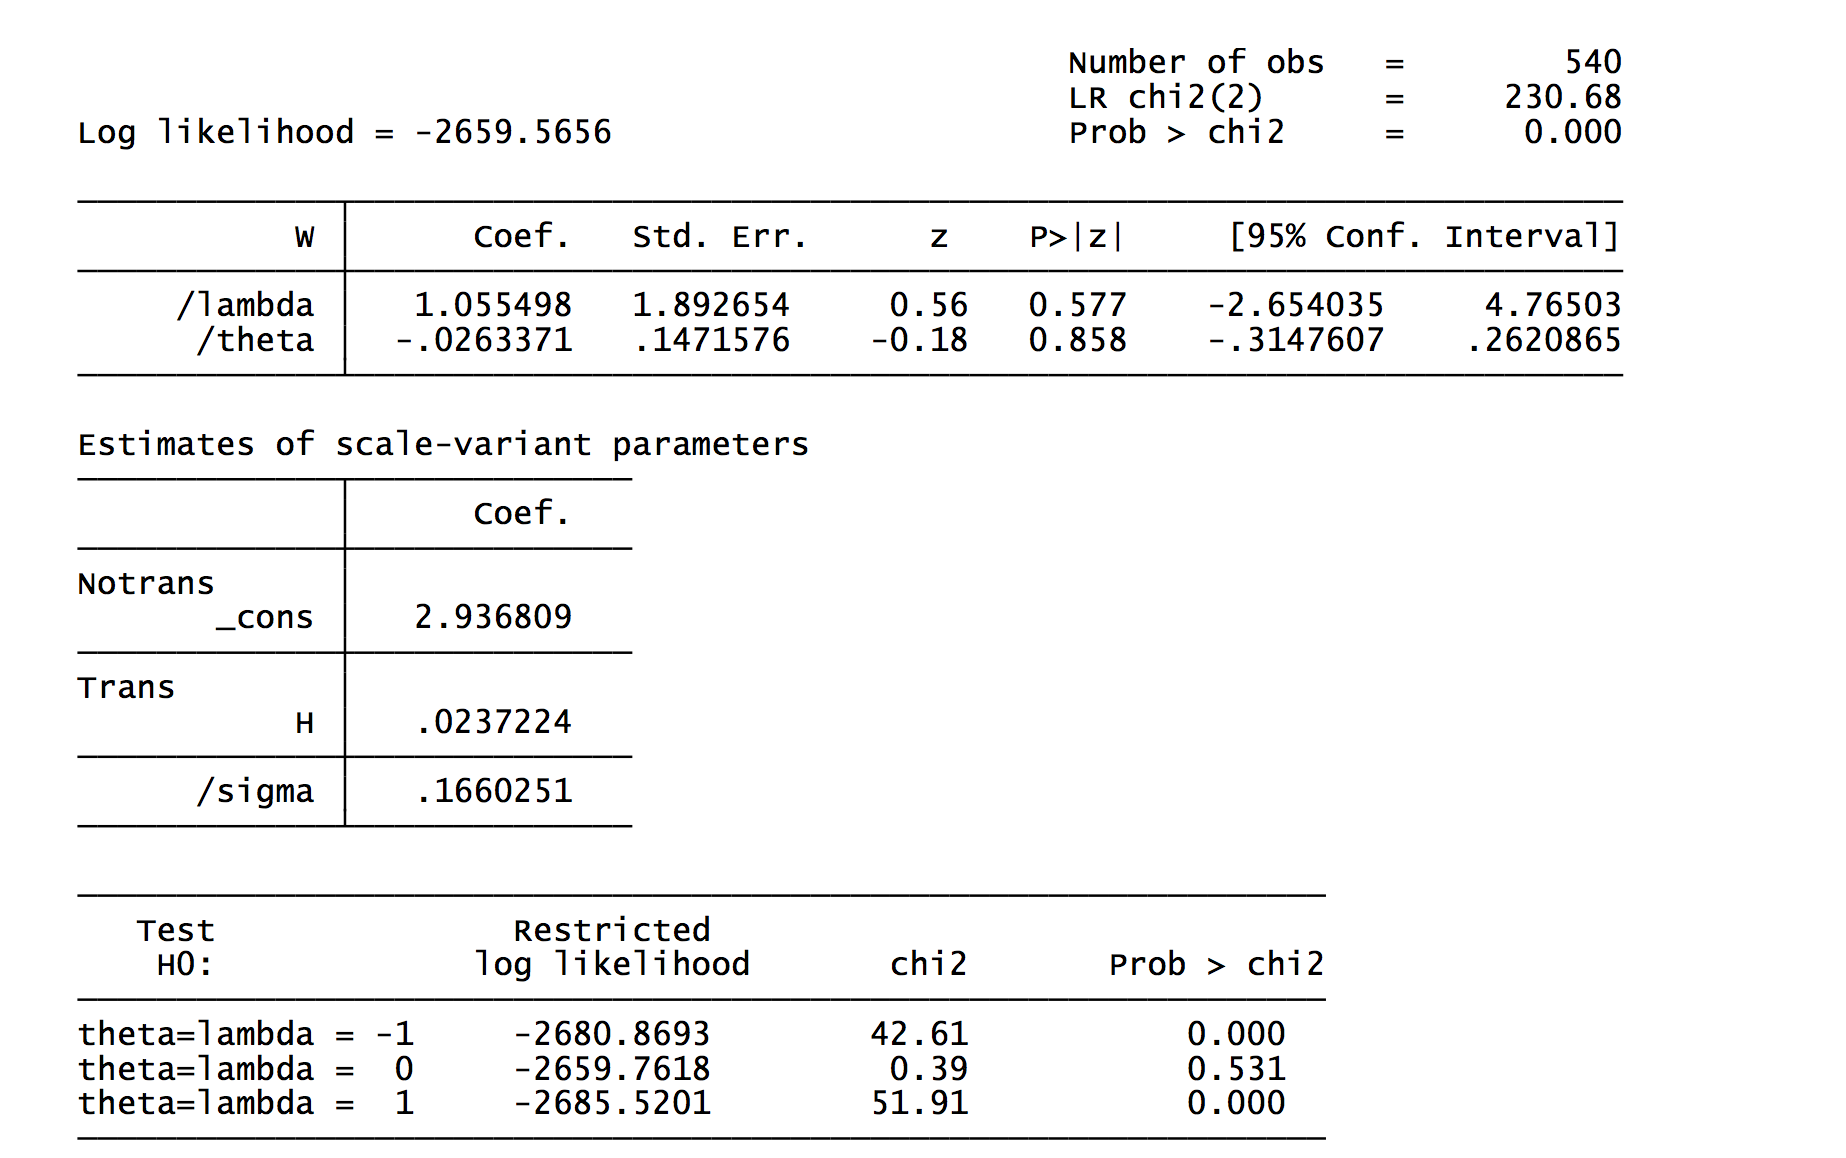
\includegraphics[width=\textwidth]{images/box_cox.png}

Какую спецификацию модели (линейную, линейную в логарифмах, полулогарифмическую) следует предпочесть и почему?

\newpage

\item По данным для  23 демократических стран оценили зависимость индекса Джини\footnote{Индекс Джини — это мера неравенства доходов. Чем выше индекс Джини, тем выше неравенство.} от ВВП на душу населения с учетом ППС (паритета покупательной способности). Затем провели тест Рамсея.

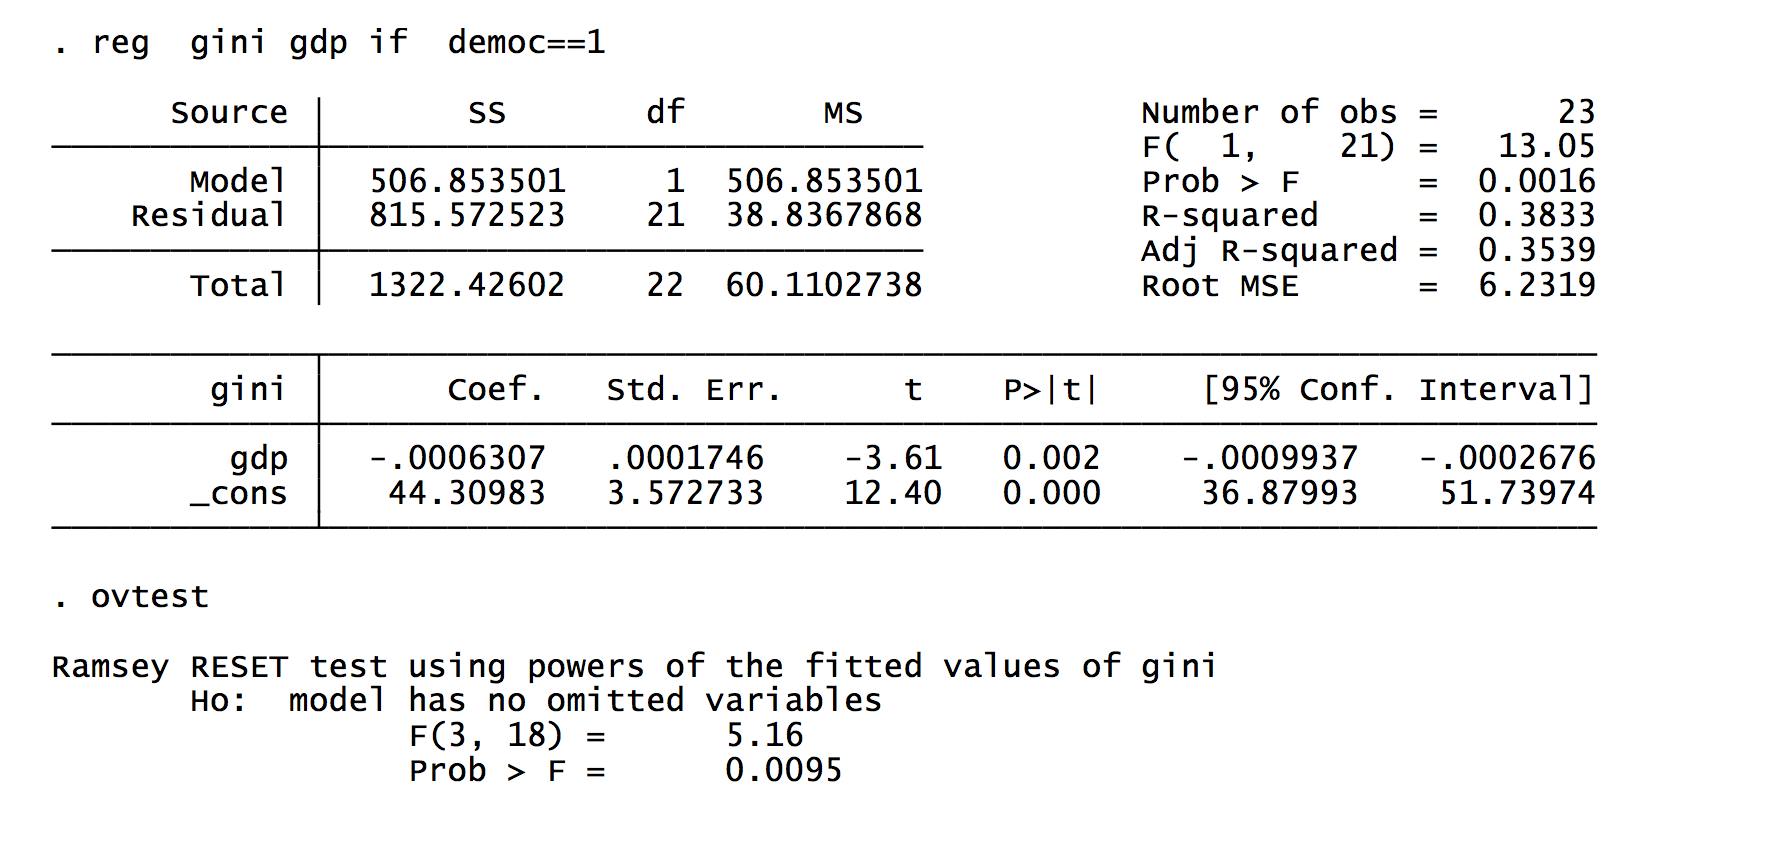
\includegraphics[width=\textwidth]{images/ramsey.png}

\begin{enumerate}
\item Сформулируйте нулевую и альтернативную гипотезу теста Рамсея
\item Опишите пошагово, как проводится тест Рамсея
\item Прокомментируйте результаты теста Рамсея
\end{enumerate}

\end{enumerate}

\newpage

Немного хинтов:

\begin{enumerate}
\item

\item
\begin{knitrout}
\definecolor{shadecolor}{rgb}{0.969, 0.969, 0.969}\color{fgcolor}\begin{kframe}
\begin{alltt}
\hlstd{y_hat} \hlkwb{<-} \hlnum{12} \hlopt{+} \hlnum{0.2} \hlopt{*} \hlnum{15}
\hlstd{se_y_hat} \hlkwb{<-} \hlnum{5} \hlopt{+} \hlnum{225} \hlopt{*} \hlnum{0.01} \hlopt{+} \hlnum{2} \hlopt{*} \hlnum{15} \hlopt{*} \hlnum{0.03}
\hlstd{se_forecast_error} \hlkwb{<-} \hlstd{se_y_hat} \hlopt{+} \hlnum{1.45}
\hlstd{t_crit} \hlkwb{<-} \hlkwd{qt}\hlstd{(}\hlnum{0.975}\hlstd{,} \hlkwc{df} \hlstd{=} \hlnum{30} \hlopt{-} \hlnum{2}\hlstd{)}
\end{alltt}
\end{kframe}
\end{knitrout}

\item
\begin{knitrout}
\definecolor{shadecolor}{rgb}{0.969, 0.969, 0.969}\color{fgcolor}\begin{kframe}
\begin{alltt}
\hlstd{t_obs} \hlkwb{<-} \hlstd{(}\hlnum{0.385}\hlopt{-}\hlnum{0.5}\hlstd{)} \hlopt{/} \hlnum{0.085}
\hlstd{t_crit} \hlkwb{<-} \hlkwd{qt}\hlstd{(}\hlnum{0.975}\hlstd{,} \hlkwc{df} \hlstd{=} \hlnum{27} \hlopt{-} \hlnum{3}\hlstd{)}
\hlstd{F_obs} \hlkwb{<-} \hlstd{(}\hlnum{0.943} \hlopt{-} \hlnum{0.74}\hlstd{)} \hlopt{/} \hlstd{(}\hlnum{1} \hlopt{-} \hlnum{0.943}\hlstd{)} \hlopt{*} \hlstd{(}\hlnum{27} \hlopt{-} \hlnum{3}\hlstd{)}
\hlstd{F_crit} \hlkwb{<-} \hlkwd{qf}\hlstd{(}\hlnum{0.95}\hlstd{,} \hlkwc{df1} \hlstd{=} \hlnum{1}\hlstd{,} \hlkwc{df2} \hlstd{=} \hlnum{27} \hlopt{-} \hlnum{3}\hlstd{)}
\end{alltt}
\end{kframe}
\end{knitrout}

\end{enumerate}


\end{document}
